\documentclass{article}

\usepackage{amsmath,amssymb}
\usepackage{tikz}
\usepackage{pgfplots}
\usepackage{xcolor}
\usepackage[left=2.1cm,right=3.1cm,bottom=3cm,footskip=0.75cm,headsep=0.5cm]{geometry}
\usepackage{enumerate}
\usepackage{enumitem}
\usepackage{marvosym}
\usepackage{tabularx}
\usepackage[amsmath,thmmarks,standard]{ntheorem}
\usepackage{mathtools}

\usepackage[utf8]{inputenc}

\renewcommand*{\arraystretch}{1.4}
\newcommand{\E}{\mathbb{E}}

\newcolumntype{L}[1]{>{\raggedright\arraybackslash}p{#1}}
\newcolumntype{R}[1]{>{\raggedleft\arraybackslash}p{#1}}
\newcolumntype{C}[1]{>{\centering\let\newline\\\arraybackslash\hspace{0pt}}m{#1}}

\DeclareMathOperator{\tr}{tr}
\DeclareMathOperator{\Var}{Var}
\DeclareMathOperator{\Cov}{Cov}
\renewcommand{\E}{\mathbb{E}}

\newtheorem{thm}{Theorem}
\newtheorem{lem}{Lemma}

\title{\textbf{Einführung in die Produktion, Hausaufgabe 5}}
\author{\textsc{Henry Haustein}}
\date{}

\begin{document}
	\maketitle
	
	\section*{Aufgabe 6}
	\begin{enumerate}[label=(\alph*)]
		\item Bei einer Mengenübersichtsstückliste sind die Mengen von alles Ausgangs- und Zwischenprodukten für 1 Endprodukt angegeben. Bei mehrstufigen Prozessen müssen diese Zahlen kumuliert werden.\\
		Die Baukastenstückliste enthält nur die Mengen der Ausgangsstoffe, die direkt für das Endprodukt benötigt werden. Bei mehrstufigen Prozessen braucht man dann mehrere Baukastenstücklisten.
		\item Graph
		\begin{center}
			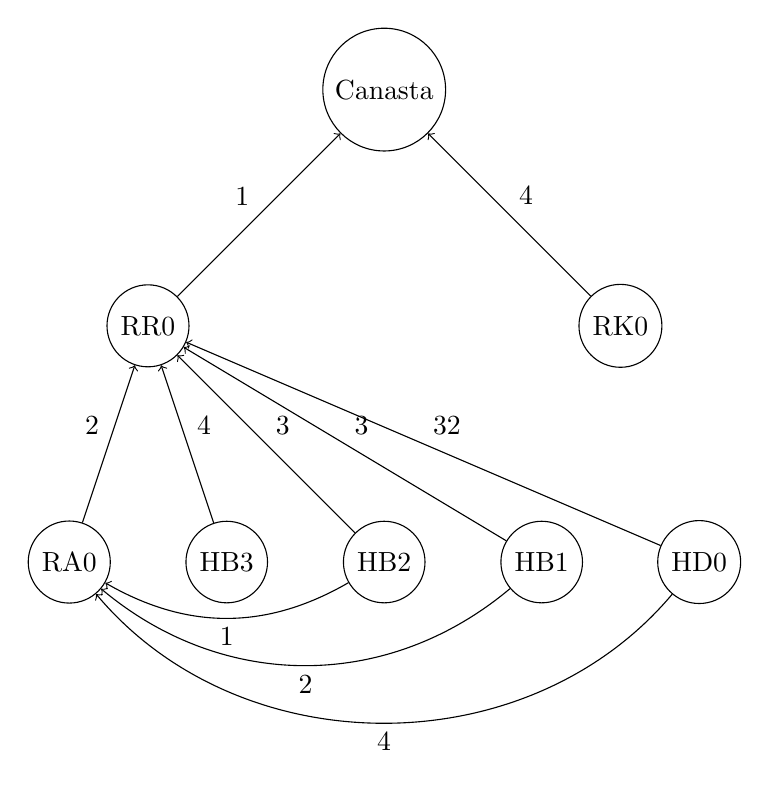
\begin{tikzpicture}
			\node[circle,draw=black, fill=white] (1) at (0,0) {Canasta};
			\node[circle,draw=black, fill=white] (2) at (-3,-3) {RR0};
			\node[circle,draw=black, fill=white] (3) at (3,-3) {RK0};
			\node[circle,draw=black, fill=white] (4) at (-4,-6) {RA0};
			\node[circle,draw=black, fill=white] (5) at (-2,-6) {HB3};
			\node[circle,draw=black, fill=white] (6) at (0,-6) {HB2};
			\node[circle,draw=black, fill=white] (7) at (2,-6) {HB1};
			\node[circle,draw=black, fill=white] (8) at (4,-6) {HD0};
			
			\draw[->] (2) to node[above left] {1} (1);
			\draw[->] (3) to node[above right] {4} (1);
			
			\draw[->] (4) to node[above left] {2} (2);
			\draw[->] (5) to node[above right] {4} (2);
			\draw[->] (6) to node[above right] {3} (2);
			\draw[->] (7) to node[above right] {3} (2);
			\draw[->] (8) to node[above right] {32} (2);
			\draw[->] (6) to[bend left=30] node[below] {1} (4);
			\draw[->] (7) to[bend left=40] node[below] {2} (4);
			\draw[->] (8) to[bend left=50] node[below] {4} (4);
			\end{tikzpicture}
		\end{center}
		\item Gozintolistenverfahren
		\begin{center}
			\begin{tabular}{c|cc|cc|cc|cc}
				& $v_1$ & $N_1$ & $v_2$ & $N_2$ & $v_3$ & $N_3$ & $v_4$ & $N_4$ \\
				\hline
				HB1 & 2 & -300 & 2 & -300 & 1 & -300 + 2400 & 0 & -300 + 2400 + 3200 \\
				HB2 & 2 & 0  & 2 & 0 & 1 & 2400 & 0 & 2400 + 1600 \\
				HB3 & 1 & 0 & 1 & 0 & 0 & 3200 & 0 & 3200 \\
				HD0 & 2 & 0 & 2 & 0 & 1 & 25600 & 0 & 25600 + 6400 \\
				RA0 & 1 & 0 & 1 & 0 & 0 & 1600 & 0 & \\
				RK0 & 1 & 200 & 0 & 200 + 3200 & 0 & 200 + 3200 & 0 & 200 + 3200 \\
				RR0 & 1 & 0 & 0 & 800 & 0 & & 0 & \\
				Canasta & 0 & 800 & 0 & & 0 & & 0 &
			\end{tabular}
		\end{center}
		Ergebnisvektor $R^T=(5300,4000,32300,32000,1600,3400,800,800)$
	\end{enumerate}
	
\end{document}